
\begin{figure*}[t]
	\begin{centering}
		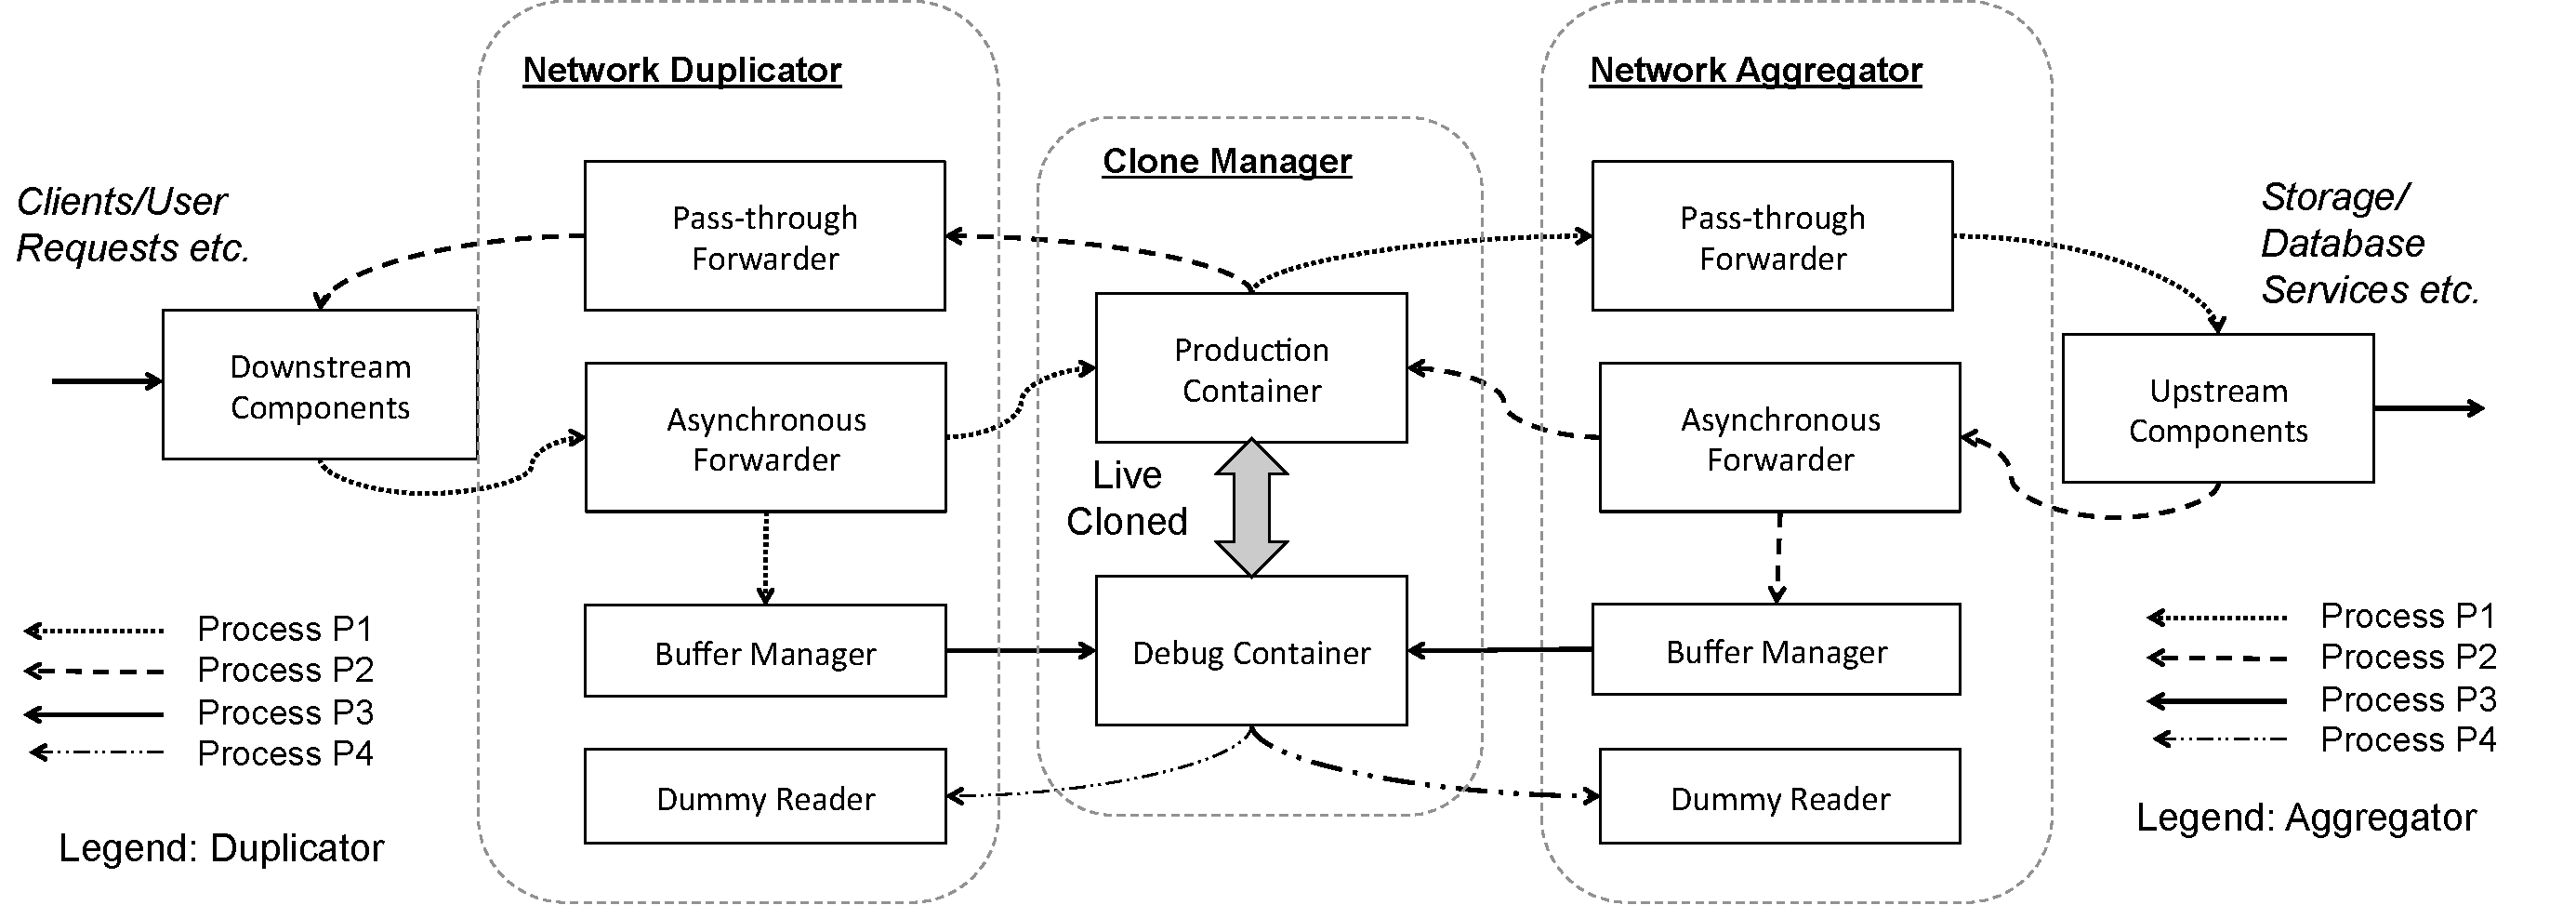
\includegraphics[width=0.99\textwidth]{parikshan/figs/arch_full.pdf}
		\caption{\textbf{High level architecture of \parikshan}, showing the main components: Network Duplicator, Network Aggregator, and Cloning Manager. The replica (debug container) is kept in sync with the master (production container) through network-level record and replay. In our evaluation, we found that this light-weight procedure was sufficient to reproduce many real bugs.}
		\label{fig:network_arch}
	\end{centering}
\end{figure*}



\section{\parikshan}
\label{sec:parikshanDesign}

In Figure~\ref{fig:network_arch}, we show the architecture of \parikshan when applied to a single mid-tier application server.
\parikshan consists of 3 modules: 
\textbf{Clone Manager}: manages ``live cloning'' between the production containers and the debug replicas, 
\textbf{Network Duplicator}: manages network traffic duplication from downstream servers to both the production and debug containers, 
and \textbf{Network Aggregator}: manages network communication from the production and debug containers to upstream servers.
The network duplicator also performs the important task of ensuring that the production and debug container executions do not diverge.
The duplicator and aggregator can be used to target multiple connected tiers of a system by duplicating traffic at the beginning and end of a workflow.
Furthermore, the aggregator module is not required if the debug-container has no upstream services. 
%At the end of this section, we also discuss the \textbf{debug window} during which we believe that the debug-container faithfully represents the execution of the production container.
%Finally, we discuss \textbf{divergence checking} which allows us to observe if the production and debug containers are still in sync.



\begin{figure}[ht]
	\begin{center}
		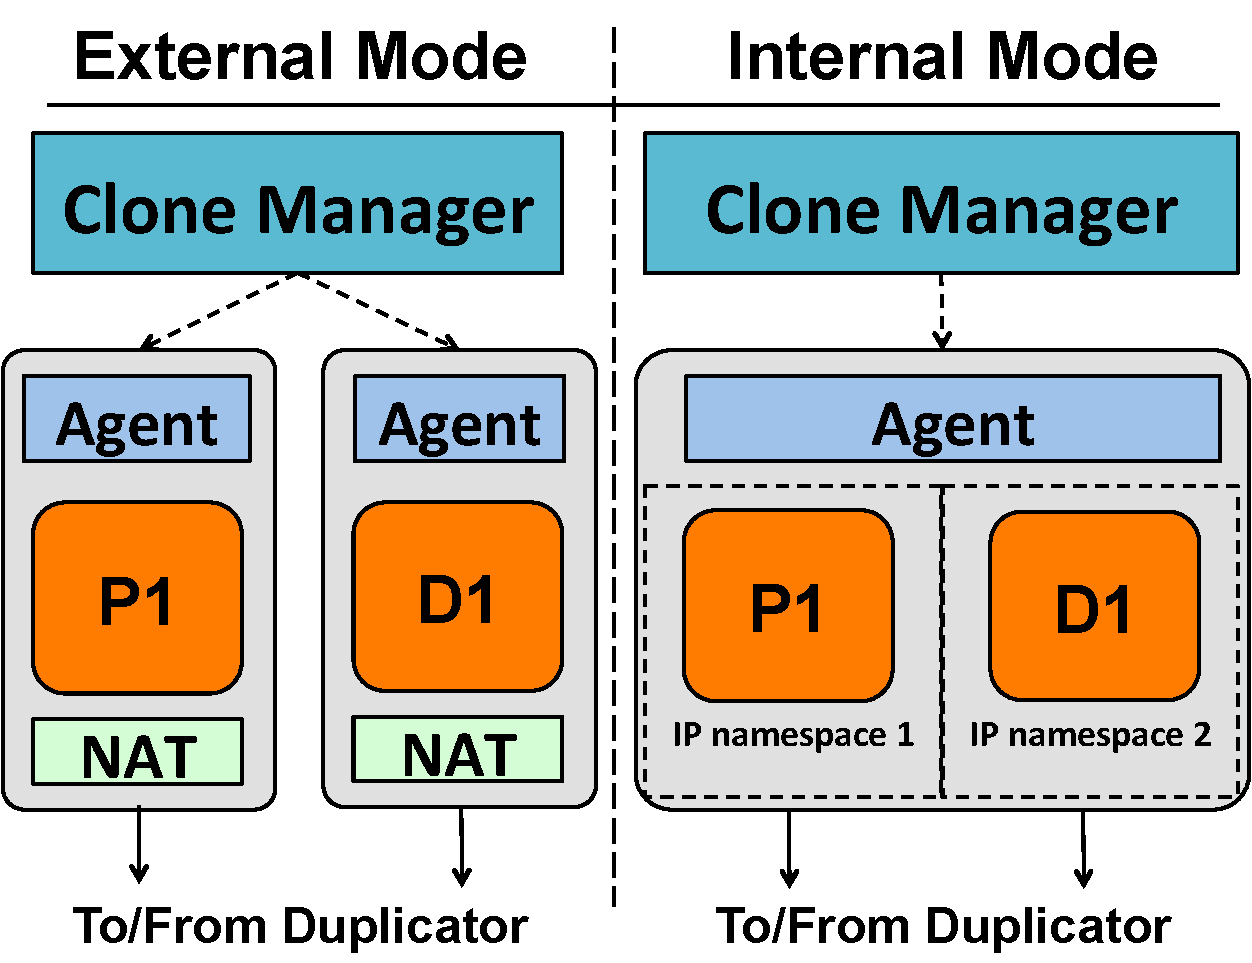
\includegraphics[width=0.9\textwidth]{parikshan/figs/ModesCloning.pdf}
		\caption{External and Internal Mode for live cloning: P1 is the production, and D1 is the debug container, the clone manager interacts with an agent which has drivers to implement live cloning.}
		\label{fig:modesCloning}
	\end{center}
\end{figure}


\subsection{Clone Manager} 
\label{sec:parikshanCloneManager}

Live migration~\cite{mirkin2008containers,clark2005live,gebhart2009dynamic} refers to the process of moving a running virtual machine or container from one server to another, without disconnecting any client or process running within the machine (this usually incurs a short or negligible suspend time). 
In contrast to live migration where the original container is destroyed, the ``Live Cloning'' process used in \parikshan requires both containers to be actively running, and be still attached to the original network.
The challenge here is to manage two containers with the same identities in the network and application domain. 
This is important, as the operating system and the application processes running in it may be configured with IP addresses, which cannot be changed on the fly.
Hence, the same network identifier should map to two separate addresses, and enable communication with no problems or slowdowns.

\noindent
We now describe two modes (see Figure~\ref{fig:modesCloning}) in which cloning has been applied, followed by the algorithm for live cloning:

\begin{itemize}
	
	\item \textbf{\textit{Internal Mode}}: In this mode, we allocate the production and debug containers to the same host node. 
	This would mean less suspend time, as the production container can be locally cloned (instead of streaming over the network). 
	Additionally, it is more cost-effective since the number of servers remain the same.
	On the other hand, co-hosting the debug and production containers could potentially have an adverse effect on the performance of the production container because of resource contention.
	Network identities in this mode are managed by encapsulating each container in separate network namespaces~\cite{netns}.
	This allows both containers to have the same IP address with different interfaces.
	The duplicator is then able to communicate to both these containers with no networking conflict.
	
	
	\item \textbf{\textit{External Mode}}: In this mode we provision an extra server as the host of our debug-container (this server can host more than one debug-container). 
	While this mechanism can have a higher overhead in terms of suspend time (dependent on workload) and requires provisioning an extra host-node, the advantage of this mechanism is that once cloned, the debug-container is totally separate and will not impact the performance of the production-container.
	We believe that external mode will be more practical in comparison to internal mode, as cloning is likely to be transient, and high network bandwidth between physical hosts can offset the slowdown in cloning performance. 
	Network identities in external mode are managed using NAT~\cite{nat} (network address translator) in both host machines. 
	Hence both containers can have the same address without any conflict.\footnote{Another additional mode can be \textit{Scaled Mode}: This can be viewed as a variant of the external mode, where we can execute debug analysis in parallel on more than one debug-containers each having its own cloned connection. This will distribute the instrumentation load and allow us to do more analysis concurrently, without overflowing the buffer. We aim to explore this in the future.}
	
\end{itemize}

Algorithm \ref{algCloning} describes the specific process for cloning some production container P1 from Host H1 to replica D1 on Host H2.


\begin{algorithm}[ht!]
	\caption{Live cloning algorithm using OpenVZ} 
	\label{algCloning}
	\begin{enumerate}[topsep=0pt,itemsep=-1ex,partopsep=1ex,parsep=1ex]
		\item Safety checks and pre-processing (ssh-copy-id operation for password-less rsync, checking pre-existing container ID's, version number etc.) 
		\item Create and synchronize file system of P1 to D1  
		\item Set up port forwarding, duplicator, and aggregator
		\item Suspend the production container P1
		\item Checkpoint \& dump the process state of P1
		\item Since step 2 and 5 are non-atomic operations, some files may be outdated.
		A second sync is run when the container is suspended to ensure P1 and D1 have the same state
		\item Resume both production and debug containers
	\end{enumerate}
\end{algorithm}

Step 6 here is the key step which determines the suspend time of cloning. It is important to understand that the live cloning process before this step does not pause the production container and is doing a synch of the file system on the fly. Step 2 ensures that the majority of the pages between the production machine and the machine containing the \debugcontainer, are in synch.
The suspend time of cloning depends on the operations happening within the container between step 2 and step 4 (the first and the second sync), as this will increase the number of dirty pages in the memory, which in turn will impact the amount of memory that needs to be copied during the suspend phase.
This suspend time can be viewed as an amortized cost in lieu of instrumentation overhead.
We evaluate the performance of live cloning in Section~\ref{sec:parikshanPerformance}.

\subsection{Network Proxy Design Description}

The network proxy duplicator and aggregator are composed of the following internal components:

\begin{itemize}[leftmargin=*]
	\item \textbf{Synchronous Passthrough}: The synchronous passthrough is a daemon that takes the input from a source port, and forwards it to a destination port. The passthrough is used for communication from the production container out to other components (which is not duplicated).
	\item \textbf{Asynchronous Forwarder}: The asynchronous forwarder is a daemon that takes the input from a source port, and forwards it to a destination port, and also to an internal buffer. The forwarding to the buffer is done in a non-blocking manner, so as to not block the network forwarding. 
	\item \textbf{Buffer Manager}: Manages a FIFO queue for data kept internally in the proxy for the debug-container.
	It records the incoming data, and forwards it a destination port. 
	\item \textbf{Dummy Reader}: This is a standalone daemon, which reads and drops packets from a source port, or optionally saves them for divergence checking (see section~\ref{sec:parikshanDivergenceChecking})
\end{itemize}

\noindent
%Next, we explain how these components are used:\\



\iffalse
\begin{figure}[ht]
	\begin{centering}
		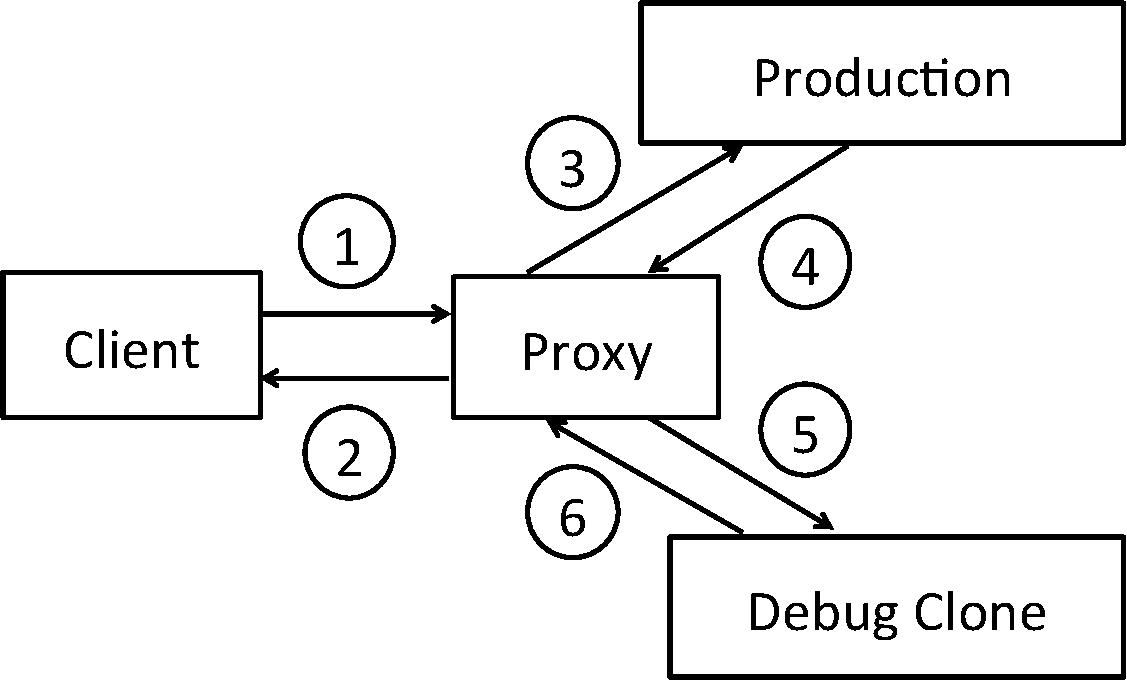
\includegraphics[width=0.9\textwidth]{parikshan/figs/network_dup.pdf}
		%    \captionsetup{justification=centering}
		\caption{Network Duplicator: Thread 1 sends traffic on links 1 and 3, Thread 2 manages links 2 and 4, Thread 3 forwards traffic on link 5, \& Thread 4 reads and drops data on link 6}
		\label{fig:duplicator}
	\end{centering}
\end{figure}
\fi



\subsubsection{Proxy Network Duplicator:} 
\label{sec:parikshanProxyDuplicator}
To successfully perform online debugging, both production and debug containers must receive the same input.
A major challenge in this process is that the production and debug container may execute at different speeds (debug will be slower than production): this will result in them being out of sync.
Additionally, we need to accept responses from both servers and drop all the traffic coming from the debug-container, while still maintaining an active connection with the client.
Hence simple port-mirroring and proxy mechanisms will not work for us. 

TCP is a connection-oriented protocol and is designed for stateful delivery and acknowledgment that each packet has been delivered.
Packet sending and receiving are blocking operations, and if either the sender or the receiver is faster than the other the send/receive operations are automatically blocked or throttled.
This can be viewed as follows: Let us assume that the client was sending packets at $X Mbps$ (link 1), and the production container was receiving/processing packets at $Y Mbps$ (link 2), where $Y<X$. 
Then automatically, the speed of link 1 and link 2 will be throttled to $Y Mbps$ per second, i.e the packet sending at the client will be throttled to accommodate the production server. 
Network throttling is a default TCP behavior to keep the sender and receiver synchronized.
However, if we also send packets to the debug-container sequentially in link 3 the performance of the production container will be dependent on the debug-container. 
If the speed of link 3 is $Z$ $Mbps$, where $Z < Y$, and $Z < X$, then the speed of link 1, and link 2 will also be throttled to $Z$ $Mbps$.
The speed of the debug container is likely to be slower than production: this may impact the performance of the production container.

Our solution is a customized TCP level proxy. 
This proxy duplicates network traffic to the debug container while maintaining the TCP session and state with the production container. 
Since it works at the TCP/IP layer, the applications are completely oblivious to it.
To understand this better let us look at Figure~\ref{fig:network_arch}: Here each incoming connection is forwarded to both the production container and the debug container . 
This is a multi-process job involving 4 parallel processes (P1-P4): In P1, the asynchronous forwarder sends data from client to the production service, while simultaneously sending it to the buffer manager in a non-blocking send.  This ensures that there is no delay in the flow to the production container because of slow-down in the debug-container.
In P2, the pass-through forwarder reads data from the production and sends it to the client (downstream component).
Process P3, then sends data from Buffer Manager to the debug container, and Process P4 uses a dummy reader, to read from the production container and drops all the packets

\iffalse
To avoid a slowdown in the production container, we use 4 threads T1, T2, T3, T4  to manage each incoming connection to the proxy.
Thread T1 forwards packets from the client to the proxy (link 1), and from the proxy to the production container (link 3). 
It then uses a non-blocking send to forward packets to an internal pipe buffer shared between thread T1, and thread T3.
Thread T2 reads the responses from the production container and forwards them to the client (link 4 and 2).
Thread T3 then reads from this piped buffer and sends the  traffic forward to the debug-container( link 5), while Thread T4, receives packets from the debug-container and drops them (link 6).
\fi

The above strategy allows for non-blocking packet forwarding and enables a key feature of \parikshan, whereby it avoids slowdowns in the debug-container to impact the production container.
We take the advantage of an in-memory buffer, which can hold requests for the debug-container, while the production container continues processing as normal.
A side-effect of this strategy is that if the speed of the debug-container is too slow compared to the packet arrival rate in the buffer, it may eventually lead to an overflow. 
We call the time taken by a connection before which the buffer overflows its \emph{debug-window}.
We discuss the implications of the \emph{debug window} in Section \ref{sec:parikshanWindow}.  

\iffalse
\begin{figure}[ht!]
	\begin{center}
		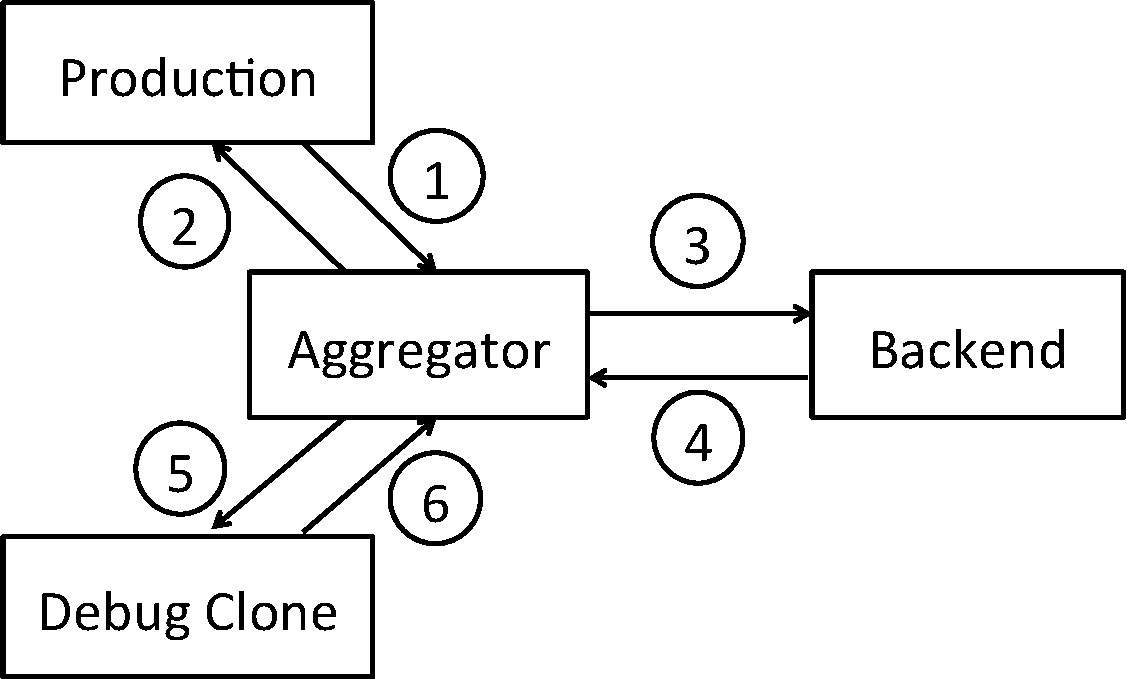
\includegraphics[width=0.9\textwidth]{parikshan/figs/aggregator.pdf}
		%    \captionsetup{justification=centering}
		\caption{Description of the Network Aggregator. Thread 1 executes step [1,3], Thread 2 step [2,4], and Thread 3 step [5], and Thread 4 step [6]}
		\label{fig:aggregator}
	\end{center}
\end{figure}
\fi


\subsubsection{Proxy Network Aggregator:}
\label{sec:parikshanProxyAggregator}
The proxy described in Section~\ref{sec:parikshanProxyDuplicator} is used to forward requests from downstream tiers to production and debug containers.
While the network duplicator duplicates incoming requests, the network aggregator manages incoming ``responses'' for requests sent from the debug container. 
Imagine if you are trying to debug a mid-tier application container, the proxy network duplicator will replicate all incoming traffic from the client to both debug and the production container. 
Both the debug container and the production, will then try to communicate further to the backend containers.
This means duplicate queries to backend servers (for instance, sending duplicate `delete' messages to MySQL), thereby leading to an inconsistent state.
Nevertheless, to have forward progress the debug-container must be able to communicate and get responses from upstream servers.
The ``proxy aggregator'' module stubs the requests from a duplicate debug container by replaying the responses sent to the production container to the debug-container and dropping all packets sent from it to upstream servers.

As shown in  Figure~\ref{fig:network_arch}, when an incoming request comes to the aggregator, it first checks if the connection is from the production container or debug container. 
In process P1, the aggregator forwards the packets to the upstream component using the pass-through forwarder.
In P2, the asynchronous forwarder sends the responses from the upstream component to the production container, and sends the response in a non-blocking manner to the internal queue in the buffer manager. 
Once again this ensures no slow-down in the responses sent to the production container.
The buffer manager then forwards the responses to the debug container (Process P3).
Finally, in process P4 a dummy reader reads all the responses from the debug container and discards them (optionally it can also save the output for comparison, this is explained further in section~\ref{sec:parikshanDivergenceChecking}).

%Responses from the backend server are sent to the aggregator (link 4), and then forwarded to the production container (link 2) and simultaneously saved in an internal queue.
%The aggregator creates an in-memory persistent inter-process FIFO queue for each connection where the responses for each of these connections are stored.
%When the corresponding connection from the duplicate debug container connects to the proxy (link 5); all packets being sent are quietly dropped. 
%The aggregator then uses the queue to send replies to the debug-container (link 6).
%In a way this is a streaming online record-and-replay, where we are recording the data in our buffer.

We assume that the production and the debug container are in the same state, and are sending the same requests. 
Hence, sending the corresponding responses from the FIFO queue instead of the backend ensures:
(a) all communications to and from the debug container are isolated from the rest of the network,
(b) the debug container gets a logical response for all it's outgoing requests, making forward progress possible,
and (c). similar to the proxy duplicator, the communications from the proxy to internal buffer is non-blocking to ensure no overhead on the production-container.

%In this design we assume that the order of incoming connections remains largely the same.
%To allow for some flexibility, we use a fuzzy checking mechanism using the hash value of the da%ta being sent to correlate the connections. 
%Each queue has a short wait time to check against incoming connections, this allows us to match slightly out of order connections.
%In case a connection cannot be correlated, we send a TCP\_FIN, to close the connection, and inform the user.
%\xxx{Does this come up? Need to talk about that as a limitation if so, or give some evidence that it doesnt otherwise}
%\yyy{you are right removed, actually I needed to update the network aggregator anyways}
%In case a connection cannot be correlated, we allow the connection to time out and send a TCP\_FIN.


\subsection{Debug Window}
\label{sec:parikshanWindow}

\parikshan's asynchronous forwarder uses an internal buffer to ensure that incoming requests proceed directly to the production container without any delay, regardless of the speed at which the debug replica processes requests.
The incoming request rate to the buffer is dependent on the client, and is limited by how fast the production container manages the requests (i.e. the production container is the rate-limiter).
The outgoing rate from the buffer is dependent on how fast the debug-container processes the requests.


Instrumentation overhead in the debug-container can potentially cause an increase in the transaction processing times in the debug-container.
As the instrumentation overhead increases, the incoming rate of requests may eventually exceed the transaction processing rate in the debug container.
If the debug container does not catch up, it can lead to a buffer overflow. 
We call the time period until buffer overflow happens the \emph{debug-window}.
The length of the \emph{debug-window} depends on the size of the buffer, the incoming request rate, and the overhead induced in the debug-container. 
For the duration of the debugging-window, we assume that the debug-container faithfully represents the production container. 
Once the buffer has overflown, the debug-container may be out of sync with the production container. 
At this stage, the production container needs to be re-cloned, so that the replica is back in sync with the production and the buffer can be discarded.
In case of frequent buffer-overflows, the buffer size needs to be increased or the instrumentation to be decreased in the replica, to allow for longer debug-windows.

The debug window size also depends on the application behavior, in particular how it launches TCP connections. 
\parikshan generates a pipe buffer for each TCP connect call, and the number of pipes are limited to the maximum number of connections allowed in the application.
Hence, buffer overflows happen only if the requests being sent in the same connection overflow the queue.
For webservers, and application servers, the debugging window size is generally not a problem, as each request is a new ``connection.''
This enables \parikshan to tolerate significant instrumentation overhead without a buffer overflow.
On the other hand, database and other session based services usually have small request sizes, but multiple requests can be sent in one session which is initiated by a user. 
In such cases, for a server receiving a heavy workload, the number of calls in a single session may eventually have a cumulative effect and cause overflows.

To further increase the \emph{debug window}, we propose load balancing debugging instrumentation overhead across multiple debug-containers, which can each get a duplicate copy of the incoming data. 
For instance, debug-container 1 could have 50\% of the instrumentation, and the rest on debug-container 2.
We believe such a strategy would significantly reduce the chance of a buffer overflow in cases where heavy instrumentation is needed.
Section~\ref{sec:parikshanTimewindowPerformance} explains in detail the behavior of the debug window, and how it is impacted by instrumentation.
\xxx{What happens when we exceed the debug window?}


\subsection{Divergence Checking}
\label{sec:parikshanDivergenceChecking}

To understand divergence between the production and the debug container, we look at the following questions:

\begin{itemize}
	\item \textbf{Can production and debug container diverge?}
	
	Database operations, web-servers, application-servers for most typical scenarios generate the same output as long as the state of the machine and the input request is the same. 
	Since the production and debug containers both start from the same state, and have received the same inputs, they should continue to keep giving the same output.
	However, it is possible for the two containers to diverge largely because of the following reasons:
	\begin{itemize}
		\item \emph{A non-deterministic bug} in the deployed application can cause different execution schedules in the production and debug-container resulting in divergent outputs. 
		If parallelism is properly handled output should still be deterministic regardless of the execution orders.
		However, in case of a concurrency bug, it is possible that the bug is triggered in one of the containers and not the other, leading to divergence.
		\item Another possible source of divergence is internal non-determinism due to timing, or random number generators. 
		For instance internal system timestamps or random generated id's could be included in the output values from an SOA application. 
		However for most applications, we believe that the semantically relevant output would not be relevant on internal non-deterministic outputs.		
		\item User instrumentation itself in the debug-container can cause divergence, by either changing the state or execution ordering etc. 
		We recommend \parikshan users to use instrumentation for monitoring purposes alone, and have largely non-invasive instrumentation, which would not lead to a state change.
		Most debugging techniques only try and understand the execution and logic flow by observing/monitoring rather than changing state.
		Additionally, service-oriented applications maintain a FIFO ordering for incoming requests. 
		Hence, transactions are executed in the order they are received. We found this to be the case in all the services we experimented on.
	\end{itemize}
	
	\item \textbf{Can we measure and monitor divergence?}
	
	To understand and capture this divergence, we offer an \textbf{\emph{optional feature}}\footnote{It is important to note that this feature is optional, and for better performance the packets can simply be dropped} in \parikshan to capture and compare the network output  of the production-container with the debug-container received in the proxy.
	Instead of discarding the network output from the debug container, we asynchronously take the hash of the output, and compare it to the production containers corresponding output.
	This gives us a black-box mechanism to check the fidelity of the replica based on its communication with external components.
	
	Divergence checking, can be customized for each application, and different fields of the output can potentially be discarded for comparing the output.
	Essentially, the degree of acceptable divergence is dependent on the application behavior, and the operator's wishes. 
	For example, an application that includes timestamps in each of its messages (i.e. is expected to have some non-determinism) could perhaps be expected to have a much higher degree of acceptable divergence than an application that should normally be returning deterministic results.
	Developers can use domain knowledge to design a better divergence checker depending on what part of the output ``must be" the same.
		
	\item \textbf{How can we manage divergence, so as to continue faithful debugging?}
	
	Once the production and debug container have diverged, \parikshan's debug replica can be re-synced with the production container to get it back to the same state.
	This process of re-syncing can be periodically repeated or triggered when divergence is discovered to make the debug-container faithfully represent the production execution.
	We discuss re-synchronization in further detail in the next section~\ref{sec:periodicSynch}
	
\end{itemize}


\subsection{Re-Synchronization}
\label{sec:periodicSynch}

As described in the last section it is possible for the production and debug containers to diverge. 
To manage this divergence, and for the debug-container to faithfully represent the production application it is necessary to re-synchronize the production container with the debug-container.
%TODO: Add cites for re-synchronization by looking for bcrw/Aftersight can also be considered an earlier implementation of something similar
Re-synchronization can be optimized by using a COW~\cite{cow} file system such as BTRFS~\cite{btrfs}, which can track deltas from the initial live clone snapshot. 
This optimizes the re-synchronization process, as the only parts of the system snapshot that need to be checked are the deltas from the last snapshot (we assume the snapshot is a synch point when the production and debug-containers were live cloned).

This process of re-synchronization can be triggered in three different ways based on operator requirements:
\begin{itemize}
	
	\item \textbf{Periodically}: Periodically check for divergence of the deltas, for the debug-container to have a high fidelity representation of the production-container.
	Periodic re-synchronization ensures higher fidelity, but may lead to un-necessary synchronizations, even though the containers have the same state.
	
	\item \textbf{Divergent Output}: Generally we care about output determinism, and as long as the output of the two containers do not diverge (see section ~\ref{sec:parikshanDivergenceChecking}), there is no need for re-synchronization.
	Once the output has diverged, the containers need to be re-synchronized for the debug-container to represent the production container. 
	To ensure such synchronization, the outputs from both containers must be tracked, which puts a recording overhead on the production system in the proxy.
	
	\item \textbf{Buffer Overflow}: To avoid having any overhead for checking divergence in the system output, we can trigger re-synchronization on buffer overflows.
	Buffer overflow is an indicator that the production and debug containers have definitely diverged.
	The debugging in this scenario is ``optimistic", as the production and debug containers could have divergent states even before the overflow.
	However unlike the other two modes, there is no overhead because of periodic synchronization, and production output recording.
	
\end{itemize}



\subsection{Implementation}
\label{sec:parikshanImplementation}
%\xxx{I feel like maybe this section is describing the evaluation environment. In which case, we need to talk about that in such a context, and still say something about implementation}
%\xxx{Where is the architecture diagram? The system diagram? What did we build? What are the modules? How do they talk to each other? What are the system requirements? Does it *only* run on Nipun's specially configured laptop?}
%\xxx{We are talking about kernel version why? Does the implemetation have anything to do with hacking on the kernel? The distro? Why are we going on about it?}
The clone-manager and the live cloning utility are built on top of the user-space container virtualization software OpenVZ~\cite{openvz}.
\parikshan extends \emph{VZCTL} 4.8~\cite{vzctl} live migration facility~\cite{mirkin2008containers}, to provide support for online cloning.
To make \textbf{live cloning} easier and faster, we used OpenVZ's \textit{ploop} devices~\cite{ploop} as the container disk layout.
The network isolation for the production container was done using Linux network namespaces~\cite{netns} and NAT~\cite{nat}.
While \parikshan is based on light-weight containers, we believe that \parikshan can easily be applied to heavier-weight, traditional virtualization software where live migration has been further optimized~\cite{liveVMprinciples,trafficliveVM}.
%The reason for choosing a container based implementation was that containers take much less resources in comparison to traditional VM's.

The network proxy duplicator and the network aggregator was implemented in C/C++.
The forwarding in the proxy is done by forking off multiple processes each handling one send/or receive a connection in a loop from a source port to a destination port.
Data from processes handling communication with the production container, is transferred to those handling communication with the debug containers using \emph{Linux Pipes}~\cite{linuxpipes}.
Pipe buffer size is a configurable input based on user-specifications.

